\documentclass[11pt,serif]{article}

\input{.plmt/plmt.tex}

\geometry{margin=2.5cm}

\usepackage[right]{lineno}
\linenumbers
\usepackage{endfloat}

\begin{document}

\thispagestyle{empty}

{\bfseries\huge Data-based, synthesis-driven: setting the agenda for computational
ecology}

\vskip 5em

\begin{flushleft}
\href{http://orcid.org/0000-0002-0735-5184}{Timothée Poisot}
~\emph{1,2,3}
\quad
\mbox{Richard LaBrie}
~\emph{1,2}
\quad
\mbox{Erin Larson}
~\emph{4}
\quad
\mbox{Anastasia Rahlin}
~\emph{5}
\end{flushleft}
\bigskip

\small
\textbf{1}:~Université de Montréal, Département de Sciences Biologiques;\quad\textbf{2}:~Groupe de Recherche Interuniversitaire en Limnologie et environnement
aquatique;\quad\textbf{3}:~Québec Centre for Biodiversity Sciences;\quad\textbf{4}:~Department of Ecology and Evolutionary Biology, Cornell University;\quad\textbf{5}:~Illinois Natural History Survey\normalsize
\vfill

Computational ecology, defined as the application of computational
thinking to ecological problems, has the potential to transform the way
ecologists think about the integration of data and models. As the
practice is gaining prominence as a way to conduct ecological research,
it is important to reflect on what its agenda could be, and how it fits
within the broader landscape. In this contribution, we suggest areas in
which empirical ecologists, modellers, and the emerging community of
computational ecologists could engage in a constructive dialogue to
build on one another expertise; specifically, about the need to make
predictions from models actionable, about the best standards to
represent ecological data, and about the proper ways to credit data
collection and data reuse. We discuss how training can be amended to
improve computational literacy.
\vskip 1em
{\small{\bfseries Keywords:}
computational ecology  - ecological synthesis  - data sharing \vskip 4em
}

\vfill

{\small%
{\ccby}\\
{\emph{This work is licensed under a %
Creative Commons Attribution 4.0 Unported License.}}%
\\
Correspondence to Timothée Poisot -- \texttt{timothee.poisot@umontreal.ca}\newline
\texttt{2017-03-02T00:00:00.000Z}
}%

\cleardoublepage

\doublespacing

Computational science happens when algorithms, software, data management
practices, and advanced research computing are put in interaction with
the explicit goal of solving ``complex'' problems. Typically, problems
are considered
\color{gray}\emph{complex}\color{black}\color{purple}complex\color{black}
when they cannot be solved appropriately with
\color{purple}mathematical\color{black} modelling
\color{purple}(\emph{i.e.} the application of mathematical models that
are not explicitely grounded\color{black} \color{purple}into empirical
data)\color{black} or data-collection only. Computational science is one
of the ways to practice computational thinking
\color{gray}({\textbf{???}}),\color{black}\color{purple}(Papert
1996),\color{black} \emph{i.e.} the feedback loop of abstracting a
problem to its core mechanisms, expressing a solution in a way that can
be automated, and using interactions between simulations and data to
refine the original problem or suggest new knowledge. Computational
approaches are commonplace in most areas of biology, to the point where
one would almost be confident that they represent a viable career path
\color{gray}({\textbf{???}}).\color{black}\color{purple}(Bourne
2011).\color{black} Data usually collected in ecological studies have
high variability, and are time-consuming, costly, and demanding to
collect. In parallel, many problems lack appropriate formal mathematical
formulations, which we need in order to construct strong, testable
hypotheses. For these reasons, computational approaches hold great
possibilities, notably to further ecological synthesis and help
decision-making \color{gray}({\textbf{???}}).\color{black}

\color{gray}{[}levi12mtd{]}\color{black}\color{purple}(Petrovskii \&
Petrovskaya 2012).\color{black}

\color{purple}Lev12\color{black} suggested that ecology (and
evolutionary biology) should continue their move towards a
\emph{marriage of theory and data}. In addition to the lack of
adequately expressed models, this effort is hampered by the fact that
data and models are often developed by different groups of scientists,
and reconciling both can be difficult. This has been suggested as one of
the reasons for which theoretical papers (defined as \emph{papers with
at least one equation in the main text}) experience a sharp deficit in
numbers of citations
\color{gray}({\textbf{???}});\color{black}\color{purple}(Fawcett \&
Higginson 2012);\color{black} this is the tragic sign that empirical
scientists do not see the value of theoretical work, which of course can
be blamed on both parties. One of the leading textbooks for the
mathematical models in ecology and evolution
\color{gray}({\textbf{???}})\color{black}\color{purple}(Otto \& Day
2007)\color{black} is more focused with algebra and calculus, and not
with the integration of models with data. Other manuals that cover the
integration of models and data tend to lean more towards statistical
models \color{gray}({\textbf{???}},
{\textbf{???}}).\color{black}\color{purple}(Bolker 2008; Soetaert \&
Herman 2008).\color{black} This paints a picture of ecology as a field
in which dynamical models and empirical data do not interact much, and
instead the literature develops in silos.

What is computational ecology? It is the application of computational
thinking to ecological problems. This defines three core characteristics
of computational ecology. First, it recognizes ecological systems as
complex and adaptive; this places a great emphasis on mathematical tools
that can handle, or even require, a certain degree of stochasticity
\color{gray}({\textbf{???}},
{\textbf{???}}).\color{black}\color{purple}(Zhang 2010,
2012).\color{black} Second, it understands that data are the final
arbiter of any simulation or model
\color{gray}({\textbf{???}});\color{black}\color{purple}(Petrovskii \&
Petrovskaya 2012);\color{black} this favours the use of data-driven
approaches and analyses
\color{gray}({\textbf{???}}).\color{black}\color{purple}(Beaumont 2010).
On this point,\color{black} \color{purple}computational approaches
differ greatly from modelling, that can often function\color{black}
\color{purple}on their own.\color{black} Finally, it accepts that some
ecological systems are too complex to be formulated in mathematical or
programmatic terms
\color{gray}({\textbf{???}});\color{black}\color{purple}(Pascual
2005);\color{black} the use of conceptual, or ``toy'' models, as long as
they can be confronted to empirical data, is preferable to ``abusing''
mathematics by describing the wrong mechanism well
\color{gray}({\textbf{???}}).\color{black}\color{purple}(May 2004). By
contrast, modelling approaches are by construction limited
to\color{black} \color{purple}problems that can be expressed in
mathematical terms.\color{black}

Ecology as a whole (and community ecology in particular) circumvented
the problem of model and data mismatch by investing in the development
and refinement of statistical models {[}see
\color{gray}{[}wart14mtc{]}\color{black}\color{purple}WarFos14\color{black}
for an excellent overview{]} and ``numerical'' approaches
\color{gray}({\textbf{???}})\color{black}\color{purple}(Legendre \&
Legendre 1998)\color{black} based on multivariate statistics. These
models are able to \emph{explain} data, but very rarely do they give
rise to new
\color{gray}predictions.\color{black}\color{purple}predictions --
despite it being a very clear priority even if we ``simply''
seek\color{black} \color{purple}to further our understanding (Houlahan
et al. 2017).\color{black} Computational ecology can fill this niche; at
the cost of a higher degree of abstraction, its integration of data and
generative models (\emph{i.e.} models that, given rules, will generate
new data) can be helpful to initiate the investigation of questions that
have not received (or perhaps cannot receive) extensive empirical
treatment, or for which usual statistical approaches fall short.

In a thought-provoking essay,
\color{gray}{[}mark17abc{]}\color{black}\color{purple}Mar17\color{black}
suggests that \emph{all biology is computational biology} -- the
rationale behind this bold statement being that integrating
computational advances, novel mathematical tools, and the usual data
from one field, has a high potential to deliver synthesis. A more
reasonable statement would be that \emph{all ecology can benefit from
computational ecology}, as long as we can understand how it interacts
with other approaches; in this paper, we attempt to situate the practice
of computational ecology within the broader landscape of ecological
research. In particular, we highlight the ways in which computational
ecology differs from, and complements, ecological modelling. We finally
move on to the currency of collaborations between different
sub-disciplines of ecologists, and discuss the need to add more
quantitative skills in ecological training.

\section{A success story: Species Distribution
Models}\label{a-success-story-species-distribution-models}

The practice known as ``species distributions modelling'' (and the
species distribution models, henceforth SDMs, it generates) is a good
example of computational practices generating novel ecological insights.
At their core, SDMs seek to model the presence or absence of a species
based on previous observations of its presence or absences, and
knowledge of the environment in which the observation was made. More
formally, SDMs can be interpreted as having the form
\(\text{P}(S | E)\)\color{purple}(or \(\text{P}(S | E=1)\) for
presence-only models),\color{black} where \(S\) denotes the presence of
a species, and \(E\) is an array of variables representing the local
state of the environment at the point where the prediction is made (the
location is represented, not by its spatial positions, but by a suite of
environmental variables).

As
\color{gray}{[}fran10msd{]}\color{black}\color{purple}Fra10\color{black}
highlights, SDMs emerged at a time where access to computers \emph{and}
the ability to effectively program them became easier. Although
ecological insights, statistical methods, and data already existed, the
ability to turn these ingredients into something predictive required
what is now called ``computational literacy'' -- the ability to
abstract, and automate, a system in order to generate predictions
through computer simulations and their validation. One of the strengths
of SDMs is that they can be used either for predictions or explanations
of where a given species occur
\color{gray}({\textbf{???}})\color{black}\color{purple}(Elith \&
Leathwick 2009)\color{black} and can be corroborated with empirical
data. To calculate \(\text{P}(S | E)\) is to make a prediction (what are
the chances of observing species \(S\) at a given location), that can be
refined, validated, or rejected based on
\color{gray}sampling.\color{black}\color{purple}cross-validation
(Hijmans 2012) or \emph{de novo}\color{black} \color{purple}field
samplig (West et al. 2016).\color{black} To understand \(E\),
\emph{i.e.} the environmental aspects that determine species presence,
is to form an explanation of a distribution that relates to the natural
history of a species.

SDMs \color{gray}exist at the interface
between\color{black}\color{purple}originated as statistical and
correlative models, and are now incorporating\color{black}
\color{purple}more\color{black} ecological theory \color{gray}and
statistical models\color{black}
\color{gray}({\textbf{???}})\color{black}\color{purple}(Austin
2002)\color{black} -- being able to integrate (abstract) ideas and
knowledge with (formal) statistical and numerical tools is a key feature
of computational thinking. In fact, one of the most recent and most
stimulating developments in the field of SDMs is to refine their
predictions not through the addition of more data, but through the
addition of more processes
\color{gray}({\textbf{???}}).\color{black}\color{purple}(Franklin
2010).\color{black} These SDMs rely on the usual statistical models, but
also on dynamical models
\color{gray}(\emph{i.e.}\color{black}\color{purple}(for
example\color{black} simulations;\color{gray}see\color{black}
\emph{e.g.}
\color{gray}{[}wisz12rbi{]}\color{black}\color{purple}WisPot12\color{black}
or
\color{gray}{[}pell13cfw{]}\color{black}\color{purple}PelRoh13\color{black}
for biotic interactions, and
\color{gray}{[}mill15ims{]}\color{black}\color{purple}MilHol15\color{black}
for movement and dispersal). What they lack in mathematical
expressiveness (\emph{i.e.} having a closed-form
\color{gray}solution,\color{black}\color{purple}solution (Borwein \&
Crandall 2013),\color{black} which is\color{gray}most\color{black} often
ruled out by the use of stochastic \color{purple}models or
agent-based\color{black} simulations), they assume to gain in predictive
ability through the explicit consideration of more realistic ecological
mechanisms \color{gray}({\textbf{???}},
{\textbf{???}}).\color{black}\color{purple}(D'Amen et al. 2017;
Staniczenko et al. 2017).\color{black} SDMs have been a success, but
there are many other areas of ecology that could be improved by a
marriage of computational ecology and empirical data.

\section{Computational ecology in its broader
landscape}\label{computational-ecology-in-its-broader-landscape}

\subsection{The four quadrats of ecological
research}\label{the-four-quadrats-of-ecological-research}

In \{fig.~\ref{fig:quadrats}\}, we propose a rough outline of four
quadrats for ecological research. The horizontal axis is based on the
degree of integration between data and models, ranging from disconnected
(for purely data-based or model-based) to highly integrated. The
vertical axis is based on the ability to \emph{document} natural
processes and their underlying mechanisms (through direct or indirect
observation of natural systems) rather than \emph{suggest} (through
focus on a reduced number of mechanisms and their interactions). A
classification this coarse is bound to be caricatural, but it serves as
an illustration of where computational ecology exists in the overall
research methodology. Because computational ecology relies on the
integration of data (if possible \emph{raw} data from observational and
manipulative experiments) and models (either statistical or
phenomenological), it can \emph{suggest} general trends through an
abstraction of the idiosyncracies of a particular system.

\begin{figure}
\centering
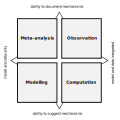
\includegraphics[width=0.50000\textwidth]{figures/fourquads.png}
\caption{An overview of four quadrats of ecological research. The
vertical axis differentiates the ability to document (by observation) or
suggest (by simulation and inference) the action of ecological
mechanisms. The horizontal axis indicates whether data and models are
connected, or not. Computational ecology constitutes one of these
quadrats, as it can bridge dynamical models with observations to further
suggest mechanisms.}\label{fig:quadrats}
\end{figure}

The specific example of predator-prey interactions should be a familiar
illustration of how the same problem can be addressed in different ways.
The classical prey--predator equations of Lotka \& Volterra are an
instance of a ``modelling'' based perspective, wherein mathematical
analysis reveals how selected parameters (rates of interactions and
growth) affect an ecologically relevant quantity (population stability
and coexistence). These models, although they have been formulated to
explain data generated through empirical observations, are disconnected
from the data themselves. In fact, this family of model lies at the
basis of a branch of ecological modelling that now exists entirely
outside of data \color{gray}({\textbf{???}}, {\textbf{???}},
{\textbf{???}}).\color{black}\color{purple}(Ackland \& Gallagher 2004;
Gyllenberg et al. 2006; Coville \& Frederic 2013). These
purely\color{black} \color{purple}mathematical models are often used to
describe trends in time series. But not\color{black} \color{purple}all
of them hold up to scrutiny when explicitely compared to empirical
data.\color{black} \color{purple}Gil73famously reports that based on the
predictions of the Lotka-Volterra\color{black} \color{purple}model,
hares in the Hudson bay are feeding on Lynx.\color{black}

By contrast
\color{gray}{[}sall11ppd{]}\color{black}\color{purple}SalKam11\color{black}
study the same issue (sustained persistence and fluctuations of
predator--prey couples through time) using a paleo-ecological
timeseries, and interpret their data in the context of predictions from
the Lotka-Volterra family of models (namely, they find support for
Lotka-Volterra-like oscillations in time). Although dynamical models and
empirical data interact in this example, they do not do so directly ;
that is, the analysis of empirical data is done within the context of a
broad family of model, but not coupled to \emph{e.g.} additional
simulations. \color{purple}A number of other\color{black}
\color{purple}models have been shown to generate predictions that
quantitatively match\color{black} \color{purple}empirical data
(Nicholson \& Bailey 1935; Beverton \& Holt 1957) -- this represents, in
our opinion, the\color{black} \color{purple}sole test of whether a
mathematical model is adapted to a particular problem and\color{black}
\color{purple}system. While models are undeniably useful to make
mechanisms interact in a\color{black} \color{purple}low-complexity
setting, it is in our opinion a grave mistake to assume
they\color{black} \color{purple}will, in and of themselves, be relevant
to empirical systems.\color{black}

Meta-analyses, such as the one by
\color{gray}{[}boln05rcm{]},\color{black}\color{purple}BolPre05,\color{black}
are instead interested in collecting the outcome of observational and
manipulative studies, and synthetizing the \emph{effects} they report.
These are often purely \emph{statistical}, in that they aggregate
significance, effect size, to measure how robust a result is across
different systems. Meta-analyses most often require a \emph{critical
mass} of pre-existing papers
\color{gray}({\textbf{???}}).\color{black}\color{purple}(Lortie et al.
2013).\color{black} Although they are irreplaceable as a tool to measure
the strength of results, they are limited by their need for primary
literature with experimental designs that are similar enough.

\subsection{Computational ecology in
context}\label{computational-ecology-in-context}

In \emph{Life on the Mississippi}, Mark Twain wrote that ``There is
something fascinating about science. One gets such wholesale returns of
conjecture out of such a trifling investment of fact''. This is a good
description of the purpose of computational ecology: in a data-limited
context, merging phenomenological models with pre-existing datasets is a
way to efficiently develop conjectures, or more appropriately, build on
our knowledge of models and data to put forward testable, quantified
hypotheses.
\color{gray}{[}pasc05cec{]}\color{black}\color{purple}Pas05\color{black}
outlines that computational ecology has a unique ability to go from the
complex (natural systems) to the simple (representations and conceptual
models), and back (testable predictions). Although the natural world is
immensely complex, it is paradoxically the high degree of model
abstraction in computational approaches that gives them generality.
Because (with the exception of a still narrow family of problems that
can be addressed by remote-sensing) \color{purple}there has been no
regime shift in\color{black} the rate at which ecological data are
collected \color{gray}is not improving,
whereas\color{black}\color{purple}-- observations from citizen
science\color{black} \color{purple}accumulate, but are highly biased by
societal preferences rather than\color{black} \color{purple}conservation
priority (Donaldson et al. 2016; Troudet et al. 2017), by proximity to
urban centers and\color{black} \color{purple}infrastructure (Geldmann et
al. 2016), \emph{as well as} by the interaction between
these\color{black} \color{purple}factors Tiago et al. (2017). On the
other hand,\color{black} our needs for testable and actionable
predictions \color{gray}increases,
refining\color{black}\color{purple}increased dramatically.
Refining\color{black} the models and further integrating them with data
is necessary.

In \{tbl.~\ref{tbl:costbenefit}\}, the quadrats of ecological approaches
are ranked in (again, approximate and arbitrary) order of cost and
effort. Ecological models make, by definition, high accuracy
predictions, but they tend to be difficult to test
\color{gray}({\textbf{???}})\color{black}\color{purple}(Rykiel
1996)\color{black} -- models relying on precise mathematical expressions
can be difficult to calibrate or parameterize. Observations (field
sampling) or manipulative approaches (micro/meso/macro-cosms, field
experiments) are highly accurate (but have also immense human and
monetary costs that limit the scale at which they can be applied). There
is simply too much nature around for us to observe, monitor, and
manipulate it all.

\hypertarget{tbl:costbenefit}{}
\begin{longtable}[]{@{}llll@{}}
\caption{\label{tbl:costbenefit}Overview of the properties of the
quadrats delineated in \{fig.~\ref{fig:quadrats}\}. Empirical
observations are the most effort-intensive way of doing ecology.
Computational approaches are ranked immediately below because the need
to maintain a computational infrastructure is incurring immense (though
often invisible) costs. Models are accurate in the limit of their
definition, and meta-analysis are accurate in the limit of the empirical
studies on which they are based.}\tabularnewline
\toprule
Approach & accuracy & testability & suitability for
prediction\tabularnewline
\midrule
\endfirsthead
\toprule
Approach & accuracy & testability & suitability for
prediction\tabularnewline
\midrule
\endhead
Empirical observation & yes & &\tabularnewline
Computational \color{purple}models\color{black} & unknown & yes &
directly\tabularnewline
\color{gray}Modelling\color{black}\color{purple}Mathematical
models\color{black} & yes &
\color{gray}no\color{black}\color{purple}variable\color{black} &
indirectly\tabularnewline
Meta-analysis & yes & no & no\tabularnewline
\bottomrule
\end{longtable}

\section{En route towards synthesis}\label{en-route-towards-synthesis}

The field of ecology as a whole needs to improve the ways in which it
can improve synthesis in order to become policy-relevant. Most of the
global policy challenges have an ecological or environmental component,
and outside of the \color{gray}socio-\(\star\) (ecological, economical,
cultural, \ldots{})\color{black}\color{purple}socio-ecological,
socio-economical, socio-cultural,\color{black} aspects, ecologists can
contribute to the mitigation or resolution of these challenges by i)
assessing our knowledge of natural systems, ii) developing methods to
produce scenarios using state-of-the-art models and tools, and iii)
communicating the output of these scenarios to impact policy-making.
\color{gray}{[}whit15ngo{]}\color{black}\color{purple}WhiSut15\color{black}
propose that this falls under the umbrella of \emph{action ecology},
\emph{i.e.} using fundamental knowledge and ecological theory to address
pressing, real-world questions.

\color{gray}{[}ragh16ca{]}\color{black}\color{purple}RagNar16\color{black}
suggest that this approach can also accommodate stakeholder knowledge
and engagement. By building models that rely on ecological concepts,
empirical data, and stakeholder feedback, they propose a
\emph{computational agroecology} program, to use computational tools in
the optimization of sustainable agricultural practices. This example
suggests that not only can computational approaches yield fundamental
research results in a short time frame, they can also be leveraged as a
tool for applied research and knowledge transfer now. The definition of
``a short time'' is highly sensitive to the context -- some predictions
can be generated using routine tools (in a matter of weeks), whereas
some require to develop novel methodologies, and may require years.
Accelerating the time to prediction will, in large part, require the
development of software that can be deployed and run more rapidly.
Overall, computational ecology is nevertheless nimble enough that it can
be used to iterate rapidly over a range of scenarios, to inform
interactions with policy makers or stakeholders in near real time.

\subsection{Mapping the domains of
collaboration}\label{mapping-the-domains-of-collaboration}

Understanding how computational ecology will fit within the broader
research landscape requires us to answer three questions: what can
computational ecology bring to the table, what are the needs of
computational ecologists, and what are the current limitations of
computational approaches that could limit their immediate applicability.
It seems, at this point, important to minimize neither the importance
nor the efficiency of sampling and collection of additional data.
Sampling is important because ecological questions, no matter how
fundamental, ought to be grounded in phenomena happening in nature, and
these are revealed by observation or manipulation of natural systems.
Sampling is efficient because it is the final arbiter: how good any
prediction is at explaining aspects of a particular empirical system is
determined by observations of this system, compared to the predictions.

Relying heavily on external information implies that computational
research is dependant on standards for data representation. The
Ecological Metadata Language
\color{gray}({\textbf{???}})\color{black}\color{purple}(Fegraus et al.
2005)\color{black} is an attempt at standardizing the way meta-data are
represented for ecological data; adherence to this standard, although it
has been shown to improve the ease of assembling large datasets from
single studies
\color{gray}({\textbf{???}}),\color{black}\color{purple}(Gil et al.
2011),\color{black} is done on a voluntary basis (and is therefore
abysmal). An alternative approach is to rely on community efforts to
pre-curate and pre-catalog ecological data, such as with the flagship
effort \emph{EcoDataRetriever}
\color{gray}({\textbf{???}}).\color{black}\color{purple}(Morris \& White
2013).\color{black} Yet even this approach is ultimately limited,
because of the human factor involved --- when the upstream data change,
they have to be re-worked into the software. A community consensus on
data representation, although unlikely, would actually solve several
problems at once. First, it would make the integration of multiple data
sources trivial. Second, it would provide clear guidelines about the
input and storage of data, thus maybe improving their currently limited
longevity \color{gray}({\textbf{???}}).\color{black}\color{purple}(Vines
et al. 2014).\color{black} Finally, it would facilitate the integration
of data and models with minimum efforts and risk of mis-communication,
since the format would be the same for all. To this extent, a recent
proposal by
\color{gray}{[}ovas17hmm{]}\color{black}\color{purple}OvaTik17\color{black}
is particularly interesting: rather than deciding on formats based on
knowledge of eco-informatics or data management best practices, why not
start from the ecological concepts, and translate them in digital
representation? This task requires a strong collaboration between
ecologists with topic expertise, ecologists with field expertise, and
those of us leaning closest to the computational part of the field.

With or without a common data format, the problem remains that we have
very limited insights into \color{purple}how\color{black} error
\color{gray}propagation of\color{black}\color{purple}in\color{black}
predictions made on synthetic datasets \color{gray}({\textbf{???}}).
There are biases\color{black}\color{purple}will\color{black}
\color{purple}propagate from an analysis to the other (Poisot et al.
2016); in a succesion of\color{black} \color{purple}predictive steps, do
errors at each step amplify, or cancel one another? Biases\color{black}
\color{purple}exist\color{black} in the underlying
data,\color{gray}biases\color{black} in the models used to generate the
predictions, and this can turn out in three possible ways. First,
predictions from these datasets accumulate bias and cannot be used.
Second, because the scale at which these predictions are expressed is
large, errors are (quantitatively) small enough to be over-ridden by the
magnitude of actual variation. Finally, in the best-case but low-realism
scenario, errors end up cancelling each other out. The best possible way
to understand how errors propagate is to validate predictions \emph{de
novo}. Model-validation methods can be used, as they are with SDMs
\color{gray}({\textbf{???}}),\color{black}\color{purple}(Hijmans
2012),\color{black} but \emph{de novo} sampling carries the additional
weight of being an independent attempt at testing the prediction.
Improved collaborations on this aspect will provide estimates of the
robustness of the predictions, in addition to highlighting the steps of
the process in which uncertainty is high --- these steps are natural
candidates for additional methodological development.

Finally, there is a need to assess how the predictions made by purely
computational approaches will be fed back into other types of research.
This is notably true when presenting these approaches to stakeholders.
One possible way to make this knowledge transfer process easier is to be
transparent about the way predictions were derived: which data were used
(with citations for credits and unique identifiers for
reproductibility), which software was used (with versions numbers and
code), and what the model / simulations do
\color{gray}({\textbf{???}}).\color{black}\color{purple}(White et al.
2013).\color{black} In short, the onus is on practitioners of
computational research to make sure we provide all the information
needed to communicate how predictions came to be.

\subsection{Establishing the currencies of
collaboration}\label{establishing-the-currencies-of-collaboration}

An important question to further the integration of computational
approaches to the workflow of ecological research is to establish
\emph{currencies} for collaborations. Both at the scale of individuals
researchers, research
\color{gray}groups,\color{black}\color{purple}group,\color{black} and
larger research communities, it is important to understand what each can
contribute to the research effort. As ecological research is expected to
be increasingly predictive and policy-relevant, and as fundamental
research tends to tackle increasingly refined and complex questions, it
is expected that research problems will become more difficult to
resolve. This is an incentive for collaborations that build on the
skills that are specific to different approaches.

In an editorial to the \emph{New England Journal of Medicine},
\color{gray}{[}long16ds{]}\color{black}\color{purple}LonDra16\color{black}
characterized scientists using previously published data as ``research
parasites'' (backlash by a large part of the scientific community caused
one of the authors to later retract the statement --
\color{gray}{[}draz16dsj{]}).\color{black}\color{purple}Dra16).\color{black}
Although community ecologists would have, anyways, realized that the
presence of parasites indicates a healthy ecosystem
\color{gray}({\textbf{???}},
{\textbf{???}}),\color{black}\color{purple}(Marcogliese 2005; Hudson et
al. 2006),\color{black} this feeling on unfair benefit for ecological
data re-analysis
\color{gray}({\textbf{???}})\color{black}\color{purple}(Mills et al.
2015)\color{black} has to be addressed. It has no empirical support:
\color{gray}{[}evan16gpc{]}\color{black}\color{purple}Eva16\color{black}
shows that the rate of data re-use in ecology is low and has a large
delay -- he found no instances of re-analysing the same data for the
same (or similar) purpose. There is a necessary delay between the moment
data are available, and the moment where they are aggregated and
re-purposed (especially considering that data are, at the earliest,
published at the same time as the paper). This delay is introduced by
the need to understand the data, see how they can be combined, develop a
research hypothesis, etc..

On the other hand, there are multiple instances of combining multiple
datasets collected at different scales, to address an entirely different
question {[}see
\color{gray}{[}gbif16gsr{]}\color{black}\color{purple}GBI16\color{black}
for an excellent showcase{]} -- it is more likely than data re-use is
done with the intent of exploring different questions. It is also worth
remembering that ecology as a whole, and macroecology and biogeography
in particular, already benefit immensely from data re-use. For example,
data collected by citizen scientists are used to generate estimates of
biodiversity distribution, but also set and refine conservation target
\color{gray}({\textbf{???}});\color{black}\color{purple}(Devictor et al.
2010);\color{black} an overwhelming majority of our knowledge of bird
richness and distribution comes from the \emph{eBird} project
\color{gray}({\textbf{???}},
{\textbf{???}}),\color{black}\color{purple}(Sullivan et al. 2009,
2014),\color{black} which is essentially fed by the unpaid work of
citizen scientists.

With this is mind, there is no tip-toeing around the fact that
computational ecologists will be \emph{data consumers}, and this data
will have to come from ecologists with active field programs (in
addition to government, industry, and citizens). Recognizing that
computational ecology \emph{needs} this data as a condition for its
continued existence and relevance should motivate the establishment of a
way to credit and recognize the role of \emph{data producers} {[}which
is discussed in
\color{gray}{[}pois16sdc{]},\color{black}\color{purple}PoiGra16,\color{black}
in particular in the context of massive dataset aggregation{]}. Data
re-users must be extremely pro-active in the establishment of crediting
mechanisms for data producers; as the availability of these data is
crucial to computational approaches, and as we do not share any of the
cost of collecting these data, it behooves us to make sure that our
research practices do not accrue a cost for our colleagues with field or
lab programs. Encouraging conversations between data producers and data
consumers about what data will be shared, when, and how databases will
be maintained will improve both collaborations and research quality.
\color{purple}In parallel, data producers can\color{black}
\color{purple}benefit from the new analytical avenues opened by advances
in computational\color{black} \color{purple}ecology.\color{black}
Research funders should develop financial incentives to these
collaborations, specifically by dedicating a part of the money to
developing and implementing sound data archival and re-use strategies,
and by encouraging researchers to re-use existing data when they exist.

\subsection{\texorpdfstring{Training
\color{purple}data-minded\color{black} ecologists\color{gray}in the
changing
landscape\color{black}}{Training data-minded ecologistsin the changing landscape}}\label{training-data-minded-ecologistsin-the-changing-landscape}

The fact that data re-use is not instantaneously convenient reveals
another piece of information about computational ecology: it relies on
different skills, and different tools than those typically used by field
ecologists. One of the most fruitful avenue for collaboration lies in
recognizing the strengths of different domains: the skills required to
assemble a dataset (taxonomic expertise, natural history knowledge,
field know-how) and the skills required to develop robust computational
studies (programming, applied mathematics) are different.
\color{purple}Because these skills are so transversal to any form of
ecological\color{black} \color{purple}research, we are confident that
they can be incorporated in any curriculum.\color{black} If anything,
this calls for increased collaboration, where these approaches are put
to work in complementarity.

\color{gray}{[}barr14lqt{]}\color{black}\color{purple}BarEza14\color{black}
highlighted the fact that professional ecologists received \emph{less}
quantitative and computational thinking that they think should be
necessary. Increasing the amount of such training does not necessarily
imply that natural history or field practice will be sacrificed on the
altar of mathematics: rather, ecology would benefit from introducing
more quantitative skills and reasoning across all courses, and
introductory ones in particular
\color{gray}({\textbf{???}}).\color{black}\color{purple}(Hoffman et al.
2016).\color{black} Instead of dividing the field further between
empirically and theoretically minded scientists, this would showcase
quantitative skills as being transversal to all questions that ecology
can address. What to teach, and how to integrate it to the existing
curriculum, does of course requires discussion and consensus building by
the community.

A related problem is that most practising ecologists are terrible role
models when it comes to showcasing good practices of data management
(because there are no incentives to do this); and data management is a
crucial step towards easier computational approaches. Even in the
minority of cases where ecologists do share their data on public
platforms, there are so few metadata that not being able to reproduce
the original study is the rule \color{gray}({\textbf{???}},
{\textbf{???}}).\color{black}\color{purple}(Roche et al. 2014,
2015).\color{black} This is a worrying trend, because data management
affects how easily research is done, regardless of whether the data are
ultimately archived. Because the volume and variety of data we can
collect tends to increase over time, and because we expect higher
standard of analysis (therefore requiring more programmatic approaches),
data management has already became a core skill for ecologists to
acquire.

This view is echoed in recent proposals.
\color{gray}{[}misl16esc{]}\color{black}\color{purple}MisHee16\color{black}
suggested that highlighting the importance of code in most ecological
studies would be a way to bring the community to adopt higher standards,
all the while de-mystifying the process of producing code.
\color{purple}As with increased mandatory data release along
manuscript\color{black} \color{purple}publication required by funding
agencies, mandatory code release would benefit a\color{black}
\color{purple}more reproductible science and how data were transformed
during the analysis.\color{black} This also requires teaching ecologists
how to evaluate the quality of the software they
\color{gray}use~({\textbf{???}}).\color{black}\color{purple}use~(Poisot
2015).\color{black} Finally,
\color{gray}{[}hamp15tos{]}\color{black}\color{purple}HamAnd15\color{black}
proposed that the ``Tao of Open Science'' would be particularly
beneficial to the entire field of ecology; as part of the important
changes in attitude, they identified the solicitation and integration of
productive feedback throughout the research process. Regardless of the
technical solution, this emphasizes the need to foster, in ecologists in
training, a culture of discussion across disciplinary
\color{purple}boundaries.\color{black}

\color{purple}All of these points can be distilled into practical
training recommendations for\color{black} \color{purple}different groups
in the community of ecologists. Classes based around lab or\color{black}
\color{purple}field experience should emphasize practical data
management skills, and\color{black} \color{purple}introduce tools that
would make the maintenance of data easier. Modelling\color{black}
\color{purple}classes, especially when concerned about purely
mathematical models, should add\color{black} \color{purple}modules on
the way these models can be integrated with empirical data.
Finally,\color{black} \color{purple}computational classes should
emphasize communication skills: what do these new\color{black}
\color{purple}tools do, and how can they be used by other fields in
ecology; but also, how do\color{black} \color{purple}we properly track
citations to data, and give credit to data producers?
Building\color{black} \color{purple}this practices into training would
ensure that the next generation of ecologists\color{black}
\color{purple}will be able to engage in a meaningful dialogue across
methodological\color{black} boundaries.

\section{Concluding remarks}\label{concluding-remarks}

None of these approaches to ecological research have any intrinsic
superiority -- in the end, direct observation and experimentation trumps
all, and serve as the validation, rejection, or refinement of
predictions derived in other ways, but lacks the scaling power to be the
only viable solution. The growing computational power, growing amount of
data, and increasing computational literacy in ecology means that
producing theory and predictions is becoming cheaper and faster
(regardless of the quality of these products). Yet the time needed to
test any prediction is not decreasing (or at least not as fast).
Computational science has resulted in the development of many tools and
approaches that can be useful to ecology, since they allow ecologists of
all kinds to wade through these predictions and data. Confronting
theoretical predictions to data is a requirement, if not the core, of
ecological synthesis; this is only possible under the conditions that
ecologists engage in meaningful dialogue across disciplines, and
recognize the currencies of their collaborations.

\color{gray}Discussion\color{black}\color{purple}Discussing\color{black}
the place of computational ecology within the broader context of the
ecological sciences will highlight areas of collaborations with other
areas of science.
\color{gray}{[}thes16aml{]}\color{black}\color{purple}The16\color{black}
makes the point that long-standing ecological problems would benefit
from being examined through a variety of machine learning techniques --
We fully concur, because these techniques usually make the most of
existing data
\color{gray}({\textbf{???}}).\color{black}\color{purple}(Halevy et al.
2009).\color{black} Reaching a point where these methods are routinely
used by ecologists will require a shift in our culture: quantitative
training is currently perceived as inadequate
\color{gray}({\textbf{???}}),\color{black}\color{purple}(Barraquand et
al. 2014),\color{black} and most graduate programs do not train ecology
students in contemporary statistics
\color{gray}({\textbf{???}}).\color{black}\color{purple}(Touchon \&
McCoy 2016).\color{black}

Ultimately, any additional data collection has its scope limited by
financial, human, and temporal constraints --- or in other words, we
need to chose what to sample, because we can't afford to sample it all.
Computational approaches, because they can work through large amounts of
data, and integrate them with models that can generate predictions,
might allow answering an all important question: what do we sample, and
where? Some rely on their ecological intuition to answer; although
computational ecologists may be deprived of such intuitions, they have
the know-how to couple data and models, and can meaningfully contribute
to this answer. Computational ecology is also remarkably cost-effective.
Although the reliance on advanced research computing incurs immense
costs (including hardware maintenance, electrical power, and training of
highly qualified personnel; these are often absorbed by local or
national consortia), it allows to generate predictions that are highly
\color{gray}testable\color{black}
\color{gray}({\textbf{???}}).\color{black}\color{purple}testable.\color{black}
Although the accuracy of these predictions is currently unknown (and
will vary on a model/study/question basis), any additional empirical
effort to \emph{validate} predictions will improve their quality,
reinforcing the need for dialogue and collaborations.

\textbf{Acknowledgements:} TP thanks Dr.~Allison Barner and Dr.~Andrew
McDonald for stimulating discussions, and the Station de Biologie des
Laurentides de l'Université de Montréal for hosting him during part of
the writing process. We thank the volunteers of Software Carpentry and
Data Carpentry, whose work contribute to improving the skills of
ecologists.

\section*{References}\label{references}
\addcontentsline{toc}{section}{References}

\hypertarget{refs}{}
\hypertarget{ref-AckGal04}{}
\textbf{Ackland \& Gallagher}. (2004). Stabilization of Large
Generalized Lotka-Volterra Foodwebs By Evolutionary Feedback. \emph{Phys
Rev Lett.} 93.

\hypertarget{ref-Aus02}{}
\textbf{Austin}. (2002). Spatial prediction of species distribution: an
interface between ecological theory and statistical modelling.
\emph{Ecological Modelling.} 157:101--18.

\hypertarget{ref-BarEza14}{}
\textbf{Barraquand et al.} (2014). Lack of quantitative training among
early-career ecologists: a survey of the problem and potential
solutions. \emph{PeerJ.} 2:e285.

\hypertarget{ref-Bea10}{}
\textbf{Beaumont}. (2010). Approximate Bayesian Computation in Evolution
and Ecology. \emph{Annual Review of Ecology, Evolution, and
Systematics.} 41:379--406.

\hypertarget{ref-BevHol57}{}
\textbf{Beverton \& Holt}. (1957). On the dynamics of exploited fish
populations. Springer Science \& Business Media;

\hypertarget{ref-Bol08}{}
\textbf{Bolker}. (2008). Ecological models and data in R. Princeton
University Press;

\hypertarget{ref-BorCra13}{}
\textbf{Borwein \& Crandall}. (2013). Closed Forms: What They Are and
Why We Care. \emph{Notices of the American Mathematical Society.} 60:50.

\hypertarget{ref-Bou11}{}
\textbf{Bourne}. (2011). Ten Simple Rules for Getting Ahead as a
Computational Biologist in Academia. \emph{PLoS Comput Biol.}
7:e1002001.

\hypertarget{ref-CovFre13}{}
\textbf{Coville \& Frederic}. (2013). Convergence To The Equilibrium In
A Lotka-Volterra Ode Competition System With Mutations. \emph{arXiv.}

\hypertarget{ref-DAMat17}{}
\textbf{D'Amen et al.} (2017). Improving spatial predictions of
taxonomic, functional and phylogenetic diversity. \emph{Journal of
Ecology.}

\hypertarget{ref-DevWhi10}{}
\textbf{Devictor et al.} (2010). Beyond scarcity: citizen science
programmes as useful tools for conservation biogeography.
\emph{Diversity and distributions.} 16:354--62.

\hypertarget{ref-DonBur16}{}
\textbf{Donaldson et al.} (2016). Taxonomic bias and international
biodiversity conservation research. \emph{FACETS.}

\hypertarget{ref-EliLea09}{}
\textbf{Elith \& Leathwick}. (2009). Species Distribution Models:
Ecological Explanation and Prediction Across Space and Time. \emph{Annu
Rev Ecol Evol Syst.} 40:677--97.

\hypertarget{ref-FawHig12}{}
\textbf{Fawcett \& Higginson}. (2012). Heavy use of equations impedes
communication among biologists. \emph{Proceedings of the National
Academy of Sciences.} 109:11735--9.

\hypertarget{ref-FegAnd05}{}
\textbf{Fegraus et al.} (2005). Maximizing the Value of Ecological Data
with Structured Metadata: An Introduction to Ecological Metadata
Language (EML) and Principles for Metadata Creation. \emph{Bulletin of
the Ecological Society of America.} 86:158--68.

\hypertarget{ref-Fra10a}{}
\textbf{Franklin}. (2010). Moving beyond static species distribution
models in support of conservation biogeography. \emph{Diversity and
Distributions.} 16:321--30.

\hypertarget{ref-GelHei16}{}
\textbf{Geldmann et al.} (2016). What determines spatial bias in citizen
science? Exploring four recording schemes with different proficiency
requirements. \emph{Diversity and Distributions.} 22:1139--49.

\hypertarget{ref-GilVan11}{}
\textbf{Gil et al.} (2011). Examples of ecological data synthesis driven
by rich metadata, and practical guidelines to use the Ecological
Metadata Language specification to this end. \emph{International Journal
of Metadata, Semantics and Ontologies.} 6:46.

\hypertarget{ref-GylYan06}{}
\textbf{Gyllenberg et al.} (2006). Limit cycles for
competitor--competitor--mutualist Lotka--Volterra systems. \emph{Physica
D: Nonlinear Phenomena.} 221:135--45.

\hypertarget{ref-HalNor09}{}
\textbf{Halevy et al.} (2009). The Unreasonable Effectiveness of Data.
\emph{IEEE Intelligent Systems.} 24:8--12.

\hypertarget{ref-Hij12}{}
\textbf{Hijmans}. (2012). Cross-validation of species distribution
models: removing spatial sorting bias and calibration with a null model.
\emph{Ecology.} 93:679--88.

\hypertarget{ref-HofLeu16}{}
\textbf{Hoffman et al.} (2016). Development and Assessment of Modules to
Integrate Quantitative Skills in Introductory Biology Courses.
\emph{Cell Biology Education.} 15:ar14--4.

\hypertarget{ref-HouMcK17}{}
\textbf{Houlahan et al.} (2017). The priority of prediction in
ecological understanding. \emph{Oikos.} 126:1--7.

\hypertarget{ref-HudDob06}{}
\textbf{Hudson et al.} (2006). Is a healthy ecosystem one that is rich
in parasites? \emph{Trends in ecology \& evolution.} 21:381--5.

\hypertarget{ref-LegLeg98}{}
\textbf{Legendre \& Legendre}. (1998). Numerical ecology. Oxford, UK:
Elsevier;

\hypertarget{ref-LorSte13}{}
\textbf{Lortie et al.} 2013 Jun. Practical interpretation of ecological
meta-analyses. PeerJ PrePrints; Report No.: e38v1.

\hypertarget{ref-Mar05}{}
\textbf{Marcogliese}. (2005). Parasites of the superorganism: Are they
indicators of ecosystem health? \emph{International journal for
parasitology.} 35:705--16.

\hypertarget{ref-May04}{}
\textbf{May}. (2004). Uses and Abuses of Mathematics in Biology.
\emph{Science.} 303:790--3.

\hypertarget{ref-MilTep15}{}
\textbf{Mills et al.} (2015). Archiving Primary Data: Solutions for
Long-Term Studies. \emph{Trends in Ecology \& Evolution.} 30:581--9.

\hypertarget{ref-MorWhi13}{}
\textbf{Morris \& White}. (2013). The EcoData Retriever: Improving
Access to Existing Ecological Data. \emph{PLoS ONE.} 8:e65848.

\hypertarget{ref-NicBai35}{}
\textbf{Nicholson \& Bailey}. (1935). The Balance of Animal
Populations.---Part I. \emph{Proceedings of the Zoological Society of
London.} 105:551--98.

\hypertarget{ref-OttDay07}{}
\textbf{Otto \& Day}. (2007). A biologist's guide to mathematical
modeling in ecology and evolution. Princeton University Press;

\hypertarget{ref-Pap96}{}
\textbf{Papert}. (1996). An exploration in the space of mathematics
educations. \emph{International Journal of Computers for Mathematical
Learning.} 1.

\hypertarget{ref-Pas05}{}
\textbf{Pascual}. (2005). Computational Ecology: From the Complex to the
Simple and Back. \emph{PLoS Comp Biol.} 1:e18.

\hypertarget{ref-PetPet12}{}
\textbf{Petrovskii \& Petrovskaya}. (2012). Computational ecology as an
emerging science. \emph{Interface Focus.} 2:241--54.

\hypertarget{ref-Poi15}{}
\textbf{Poisot}. (2015). Best publishing practices to improve user
confidence in scientific software. \emph{Ideas in Ecology and
Evolution.} 8.

\hypertarget{ref-PoiGra16}{}
\textbf{Poisot et al.} (2016). Synthetic datasets and community tools
for the rapid testing of ecological hypotheses. \emph{Ecography.}
39:402--8.

\hypertarget{ref-RocKru15}{}
\textbf{Roche et al.} (2015). Public Data Archiving in Ecology and
Evolution: How Well Are We Doing? \emph{PLOS Biology.} 13:e1002295.

\hypertarget{ref-RocLan14}{}
\textbf{Roche et al.} (2014). Troubleshooting Public Data Archiving:
Suggestions to Increase Participation. Eisen, ed. \emph{PLoS Biology.}
12:e1001779.

\hypertarget{ref-Ryk96}{}
\textbf{Rykiel}. (1996). Testing ecological models: the meaning of
validation. \emph{Ecological Modelling.} 90:229--44.

\hypertarget{ref-SoeHer08}{}
\textbf{Soetaert \& Herman}. (2008). A Practical Guide to Ecological
Modelling: Using R as a Simulation Platform. Springer Verlag;

\hypertarget{ref-StaSiv17}{}
\textbf{Staniczenko et al.} (2017). Linking macroecology and community
ecology: refining predictions of species distributions using biotic
interaction networks. \emph{Ecology Letters.}:n/a--a.

\hypertarget{ref-SulAyc14}{}
\textbf{Sullivan et al.} (2014). The eBird enterprise: an integrated
approach to development and application of citizen science.
\emph{Biological Conservation.} 169:31--40.

\hypertarget{ref-SulWoo09}{}
\textbf{Sullivan et al.} (2009). eBird: A citizen-based bird observation
network in the biological sciences. \emph{Biological Conservation.}
142:2282--92.

\hypertarget{ref-TiaCei17}{}
\textbf{Tiago et al.} (2017). Spatial distribution of citizen science
casuistic observations for different taxonomic groups. \emph{Scientific
Reports.} 7:12832.

\hypertarget{ref-TouMcC16}{}
\textbf{Touchon \& McCoy}. (2016). The mismatch between current
statistical practice and doctoral training in ecology. \emph{Ecosphere.}
7:e01394.

\hypertarget{ref-TroGra17}{}
\textbf{Troudet et al.} (2017). Taxonomic bias in biodiversity data and
societal preferences. \emph{Scientific Reports.} 7:9132.

\hypertarget{ref-VinAlb14}{}
\textbf{Vines et al.} (2014). The Availability of Research Data Declines
Rapidly with Article Age. \emph{Current Biology.} 24:94--7.

\hypertarget{ref-WesKum16}{}
\textbf{West et al.} (2016). Field validation of an invasive species
Maxent model. \emph{Ecological Informatics.} 36:126--34.

\hypertarget{ref-WhiBal13}{}
\textbf{White et al.} (2013). Nine simple ways to make it easier to
(re)use your data. \emph{Ideas in Ecology and Evolution.} 6.

\hypertarget{ref-Zha10}{}
\textbf{Zhang}. (2010). Computational ecology: artificial neural
networks and their applications. Singapore: World Scientific Publ;

\hypertarget{ref-Zha12}{}
\textbf{Zhang}. (2012). Computational ecology: graphs, networks and
agent-based modeling. New Jersey: World Scientific;

\end{document}
